\documentclass[11pt,twocolumn]{article}
\setlength{\columnsep}{1cm}
\usepackage[margin=1in]{geometry}
\usepackage{enumerate}
\usepackage[dvipsnames]{xcolor}
\definecolor{Navy}{HTML}{000080}
\usepackage{hyperref}
\hypersetup{
    colorlinks=true,
    linkcolor=Navy,
    filecolor=magenta,
    urlcolor=cyan,
}
\usepackage{graphicx}
\usepackage{wrapfig}
\graphicspath{ {userStudyImgs/} }

\title{PurlPal: A Hands-Free Knitting Tool}
\author{Laura Eckman $<$leckman@mit.edu$>$}
\date{6.835 Spring 2017}

\begin{document}

\maketitle

\section{Introduction} \label{intro}

When knitters work on complex patterns\footnote{For those unfamiliar with knitting, a glossary of essential terms is available in section \ref{terms}.
}, they often repeat a certain row or series of rows before switching to a new section.
This adds an additional layer of cognitive overhead to knitting - not only do these artists need to remember the particular stitch sequence for their row, they also have to remember which row they are working.
For example, a knitter might have to remember that she is on the 6th row of an 8-row section, and she needs to repeat the section 3 more times before moving to the next part of the pattern.
At the same time, she may be counting stitches in the row (``on stitch 25, purl 2, then keep knitting'').
Keeping track of these two competing number streams is very difficult - any further distractions could cause someone to forget which row or repeat they are on.
Mistaking something this simple can lead to huge problems in the finished work:
getting the number of repeats wrong could lead to a sweater that is much too narrow or wide, and
mixing up rows could lead to unsightly mistakes in the finished piece.
Furthermore, fixing entire rows in a knitted project is exceptionally time consuming because all subsequent work has to be unraveled before the mistake can be resolved - imagine having to delete the entire body of a paper to fix an incorrect sentence in the introduction, then painstakingly retyping all of the correct work you had already completed.
For these reasons, knitters are very interested in solutions that minimize cognitive overhead while facilitating accurate row tracking.

This paper introduces PurlPal, a website that uses hands-free interactions to keep track of an artist's place in their pattern while they knit.
PurlPal allows for rich interactions with knitting patterns by highlighting the current stitch and row as a user knits.
The system uses speech recognition so users can issue voice commands to navigate through the pattern rather than interrupting their work to manually update row count.
Additionally, when equipped with a LeapMotion sensor, PurlPal can automatically detect knit and purl stitches to track a user's progress through the pattern without any explicit input at all.
PurlPal aims to revolutionize knitting by providing a tool for pattern tracking that interferes minimally with artists' actual work.

\section{Interface Design} \label{design}

\subsection{Previous Work} \label{prev}

Given the severity of row-wide mistakes in knitted projects, a number of potential tracking solutions already exist.

\subsubsection{Pattern Annotation} \label{annotation}

The simplest tool for row tracking involves highlighting or tallying rows directly on the pattern or on a spare sheet of paper.
This technique requires no specialized equipment, but does require that a knitter has the pattern handy whenever they are working.
Furthermore, if the annotated paper is lost, so is all tracking knowledge.

\subsubsection{Simple Counter} \label{counters}

A very common tool is a simple row counter, either mechanical or digital. They are popular because of their portability and affordability.

\textbf{Mechanical Counters} (Figure \ref{mechanical}) are convenient because they can slide onto knitting needles and thus always are kept with the project, reducing the potential for loss.
Furthermore, they can count backwards when returning to fix a mistake by simply turning the dial the opposite direction.
\begin{figure}
  \begin{center}
    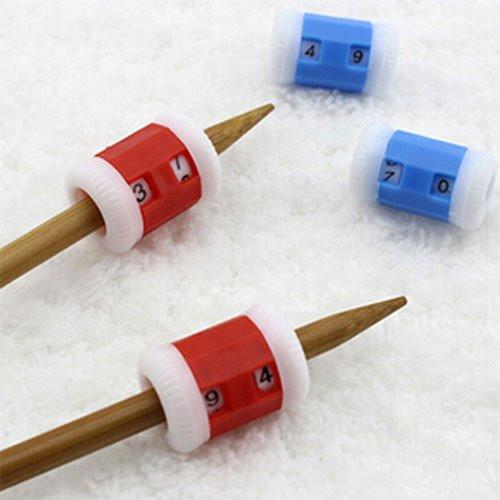
\includegraphics[width=1.5in]{rowCounter}
    \caption{A mechanical counter} \label{mechanical}
  \end{center}
\end{figure}

\textbf{Digital Counters} (Figure \ref{digital}) attach to a knitter's finger like a ring.
This makes them more practical for patterns on circular needles, where a mechanical counter would get in the way.
They are also suitable for longer patterns since they can often handle counts up to 4 digits.
At the same time, they lack the benefits of mechanical counters - they are kept separately from the rest of the project, and there is no easy way to decrement count except for fully resetting.
\begin{figure}
  \begin{center}
    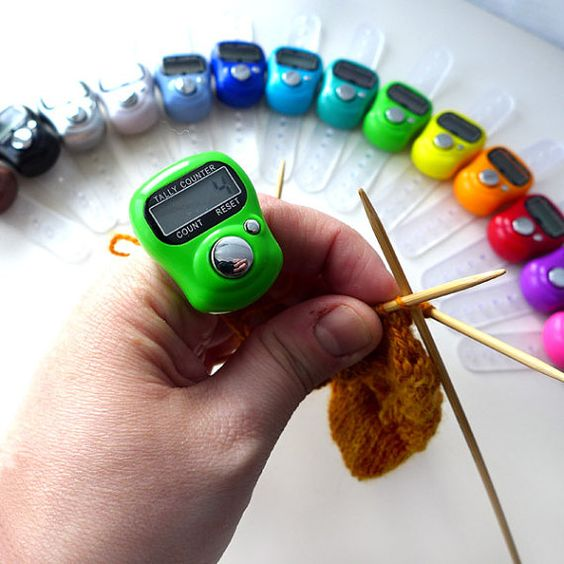
\includegraphics[width=1.5in]{digitalCounter}
    \caption{A digital counter} \label{digital}
  \end{center}
\end{figure}

Basic counters are quite handy for keeping track of rows, but knitters still have to remember how many rows or repeats exist before switching sections.
After all, it does no good for a knitter to know which row she is on if she cannot remember where the pattern changes.

\subsubsection{Existing Software}

There are three types of software currently utilized by knitters.

The first comprises standard PDF readers that allow for highlighting and annotation.
These programs effectively function as digital replacements for basic pattern annotation (\ref{annotation}).

The second type of software includes basic counter applications.
Some of these counters are marketed as knitting-specific, but in the end they are all basic tallying programs that have no additional features to support knitters.
Like the PDF readers, these tools are simply software versions of a tool that already exists.
Here, these apps function as replacements for the basic counters described previously (\ref{counters}).

The third type of software available for knitters is somewhat more promising in design.
A few pattern-tracking mobile applications have been developed that combine pattern reading from PDFs and a tallying counter.
They also allow knitters to make notes, save their place, and even upload pictures.
Problematically, however, the interfaces to these applications are cluttered, offer limited functionality in their ``free'' versions, and are very difficult to learn.

\subsubsection{Overall Inefficiencies}

The major drawback across all of these potential solutions is that they require the use of the knitter's hands.
Since knitters hold their work, requiring manual input is at minimum inefficient because it forces users to put down their project, do some other task, and then pick up their project to resume.
In the worst case, this type of input can introduce new possibilities for mistakes: perhaps a loose stitch slides off the needle or a more complex project accidentally gets turned inside-out when picking the project back up.
Another common problem is that each of these solutions immediately fails if the knitter forgets to update it.

\subsection{System Goals} \label{goals}

Building on the inadequacies of existing solutions, the primary design goals of PurlPal are simplicity and efficient interactions.
The system should be natural to use across all modalities and easy to learn.
Furthermore, redundancy should be built in so users are not pigeonholed into using a certain functionality in one way.
Given the lack of perfect reliability in speech-based or motion-based interaction, users could become quickly frustrated if they could only perform a certain action by interacting in those modalities.

\subsection{Original Plan} \label{plan}

In the original proposal, PurlPal was designed to track knit and purl stitches based on movements of the right hand while a user knitted in the English style.
The LeapMotion sensor would be placed on a lap desk and oriented to point upwards at the knitting.

Progress was displayed on a charted pattern, with the current row and stitch highlighted.
When tracking failed, users could navigate forward in the pattern by using speech commands like ``next row'' and ``next stitch'', as well as clicking provided buttons with the same functionality.
Users could also ``reset'' the pattern back to the very beginning.
As the current row and current stitch changed, the pattern highlighting updated to reflect that.

\subsection{Pivots} \label{pivots}

\subsubsection{LeapMotion Tracking} \label{pivotTracking}
Originally, I had planned to use hand tracking with the LeapMotion sensor pointed upwards, and I had intended to focus on the English knitting style, which involves more exaggerated hand movements.
I managed to develop a program that very reliably tracked the hand motions involved in a single knit or purl, based on the location of a knitter's right index finger.
However, this program failed miserably at any sort of recognition as soon as the knitter was holding a needle - the long, thin needles were either recognized as additional fingers or covered up real fingers.
To try to fix the problem, I changed the recognition to track the base of the thumb and moved the sensor closer to the knitter's body in hopes that this setup would avoid occlusion.
Even though I was able to get the same recognition accuracy on just the hand motions as the initial implementation, the program still refused to track any stitches at all when actually holding a needle.

Finally, I decided to use the LeapMotion in tool-tracking mode, which detects just the outermost tip of the right needle.
In order to get enough movement to discern stitches, I switched my focus to recognizing knit and purl stitches in the Continental style, where the right needle moves more.
I also repositioned the sensor to rest sideways against a laptop screen, pointed at the knitter instead of upwards at their work.

While this pivot enabled me to go from 0\% recognition capabilities to roughly 80\% recognition under ideal use, it also presented the most significant challenges of the project.
The tool-tracking mode and associated \texttt{Tool} API is deprecated, and the documentation that does exist is not directly applicable to the JavaScript SDK.
To get recognition to work in this way, I had to spend a lot of time investigating the \texttt{Tool} object's properties and performing small experiments to see how they varied with the motion of the knitting needle.

\subsubsection{Patterns} \label{pat-pivot}

Originally, I designed the patterns to be read left to right, top to bottom - like a book.
The chart was organized as a grid of symbols, with ``\texttt{V}'' for knit stitches and ``\texttt{-}'' for purl stitches, enabling recognition at a glance.
This made sense to me and other knitters unfamiliar with charted patterns because it is the same way written patterns are formatted.
While keeping this display format for simple patterns probably would have been fine, during my user testing (\ref{feedback}) some users pointed me towards a standard format for more complicated lace knitting.

\begin{figure}
  \begin{center}
    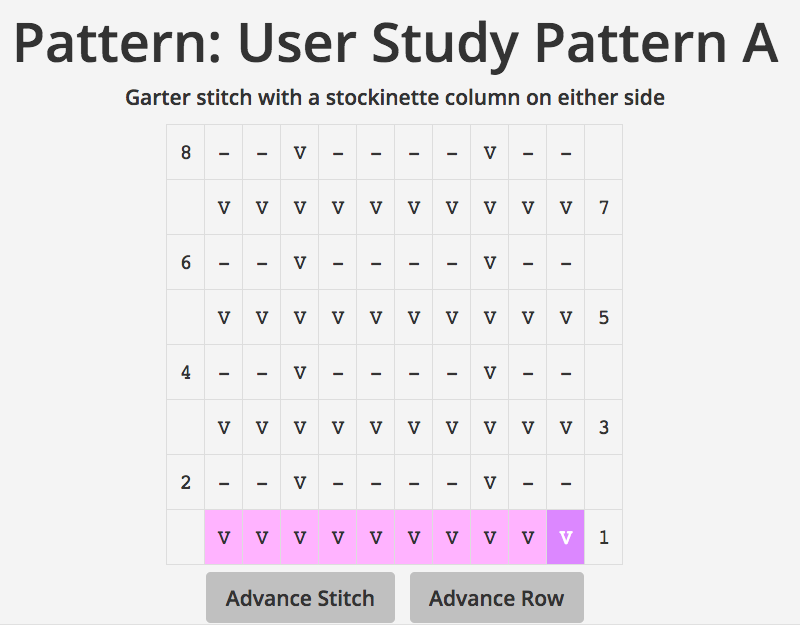
\includegraphics[width=2.25in]{finalCharted}

    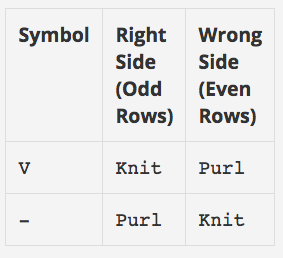
\includegraphics[width=1.25in]{sideKey}
    \caption{Default Chart Display \& Key} \label{finalCharted}
  \end{center}
\end{figure}

Since artists that often knit with charts are used to this very particular format, which starts in the bottom right corner and moves across each row and then up, I chose to change my display format to match (Figure \ref{finalCharted}).
This sets up the system for success by ensuring it will be compatible with the expected display of even the most complicated charts.
To further increase learnability in response to user commands (\ref{feedback}), I additionally added a key for the chart in the sidebar.

Furthermore, given the revelation that preferences between written and charted patterns are strongly held and most novices knit exclusively from knitting pattern (\ref{metrics}),
I moved away from my initial desire to have a single pattern display option and pivoted to provide two displays: a charted pattern (Figure \ref{finalCharted}) and a written pattern (Figure \ref{finalWritten}).
\begin{figure}
  \begin{center}
    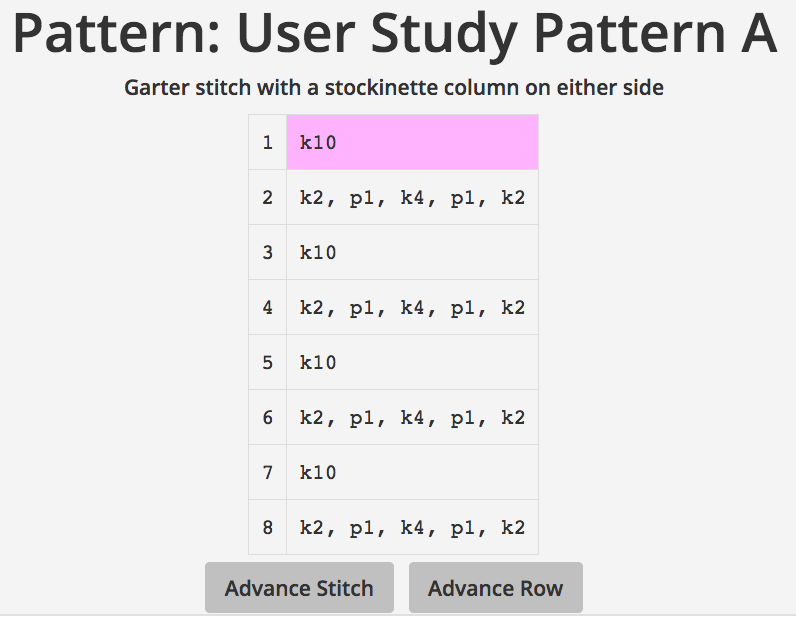
\includegraphics[width=2.25in]{finalWritten}
    \caption{Written Pattern Display} \label{finalWritten}
  \end{center}
\end{figure}
Where my initial pattern formulation was somewhat of a compromise between the left-right up-down nature of written patterns and the visual representation of charts,
the new representation does not try to alter what knitters are used to and simply provides both options as they exist in the rest of the knitting world.
Hopefully, this will also increase learnability of the system because knitters will already be familiar with at least one of the provided pattern display options.

From this pivot, I learned not to reinvent the wheel - I quite liked the hybrid chart system I devised, but it was confusing to users who were already used to seeing patterns displayed a certain way.

\subsection{Final Implementation} \label{implementation}

\subsubsection{Display}

The final interface of PurlPal shows the pattern (charted by default, as shown in Figure \ref{finalCharted}) with the first row and first stitch in that row highlighted on initial load.

\subsubsection{Manual Navigation} \label{manNav}

Under the chart, there are two buttons to \textsc{Advance Row} or \textsc{Advance Stitch} within the row.
These buttons are left conspicuous so users (a) know the basic operations available on a pattern and (b) have easy clickable options if voice or motion recognition fails.
Furthermore, the button titles double as reminders of speech commands.
A more hidden feature allows users to double-click on any cell in the pattern to select that as the current stitch and row.
A message on hover lets users know that these cells are clickable and what the effect is.

\subsubsection{Speech Navigation} \label{speechNav}

PurlPal supports two kinds of voice commands, \textsc{basic} and \textsc{smart}.

\textsc{Basic} commands always do the same thing, regardless of the context in which they are said.
This set of commands includes things like ``Next Stitch'' and ``Next Row'' for navigation, as well as commands like ``Calibrate'' for interacting with the LeapMotion detection.
Redundancy is built in - ``Advance Stitch'' and ``Move Forward'' also map to the same functionality as ``Next Stitch''.
The way the code implements this redundancy also makes it simple to add further commands, either to include a new homophone that's mistakenly recognized or to allow user-defined commands.

\textsc{Smart} commands are context-dependent.
For example, ``Go Back'' behaves as follows:
\begin{itemize}
  \item If the user is on the first, second, or third stitch of the row, the selected stitch jumps back to the beginning of the row.
  \item Otherwise, the selected stitch moves back one.
\end{itemize}
More specific \textsc{Basic} commands are available for each interpretation of the \textsc{Smart} commands.
Here, ``reset row'' accomplishes the first option deterministically, and ``back one stitch'' accomplishes the second.
While resetting to the beginning of the pattern was always available with speech command ``reset pattern'', navigating backwards through the pattern in smaller increments was added in response to user comments (\ref{feedback}) that they would prefer to continue interacting via speech if they wanted to move backwards, as opposed to putting down their work to double click on the previous cell.

A full list of supported speech commands is available in Section \ref{speech-commands}.

\subsubsection{Motion Navigation} \label{leapNav}

\textbf{Calibration Process} - For motion detection to be effective across different users and across different usage conditions, PurlPal dynamically calibrates to the position of the knitter automatically on initial load.
To calibrate, the knitter holds their needles as if to knit for roughly 3 seconds while the system calculates the average vertical position of the right needle tip over 50 frames.
This value is taken as the ``resting'' position of the knitter and all detection parameters are expressed relative to this value.
\\ \\
\textbf{Detection Parameters} \\
\texttt{sampleFrequency} tells the program whether or not to act on a newly reported frame - for example, \texttt{sampleFrequency = 4} tells the program to only process every 4th frame.
Higher values reduce noise and free up the JavaScript thread so other scripts, like speech recognition, can run more frequently.
Lower values sample more often and thus make more information available to the program. \\
\texttt{y\_threshold} gives the vertical margin around the user's calibrated ``resting'' position that is considered neutral.
Stitches are registered\footnote{A video demo of stitch detection is available at https://www.youtube.com/watch?v=nTWYvqi57DY.} by detecting the knitting needle rising to this margin above the resting position and then descending below the neutral zone.
Lower values require less movement to register stitches but makes the system more prone to over-counting.
Higher values are less prone to these false positives but require more exaggerated movements by the knitter.
In the final implementation, the empirically derived value of \texttt{y\_threshold} is 8.

\subsubsection{System Feedback} \label{aud-feedback}

Following user evaluations (\ref{feedback}), auditory feedback was implemented to allow users to get information from the system without looking at it.

First, voice inquiries were added.
The system can answer questions like ``What's this stitch?'' or ``How do I do it?'' by referring to the knitter's current row and stitch information and returning the name or instructions associated with the highlighted cell.

Second, short ``click'' sounds were added when the system advances through the pattern.
This signal lets users know their voice command or motion input has been recognized, even if they are looking at their knitting or have a different tab open in their web browser instead of visually attending to PurlPal.
For added information, a higher-pitched sound is played when the next stitch to be worked is different from the one just completed - i.e.\ moving from a knit to a purl.
This subtle cue can remind knitters when changes are coming in a relatively unobtrusive way.

\section{User Evaluation} \label{eval}

\subsection{Study Design}

\subsubsection{Quantitative Evaluation}

Two patterns were involved in the experiment (Figure \ref{patterns}).
Pattern A was 4 rows of 10 stitches each where the 3rd and 7th stitches formed a stockinette column.
Pattern B was 4 rows of 10 stitches each where the first two and last two stitches formed a garter border.

\begin{figure} %this figure will be at the right
    \centering
    \includegraphics[width=2.5in]{patterns}
    \caption{Pattern A (left) and Pattern B (right), as presented to participants.} \label{patterns}
\end{figure}


Participants recruited from a knitting group on campus began knitting in ``Continental'' style with pattern A or B.
Patterns were chosen with equal probability in order to counterbalance any effects of an unintentionally ``harder'' pattern.
For both conditions, the number of changes in visual attention from looking at the screen to looking at their knitting were noted.
The number of times the participant made a mistake and went back to correct it was also noted.
Furthermore, the participants were timed from their first completed stitch until they finished the section or stopped knitting.

Difficulties participants had in utilizing certain functionality in PurlPal and instances when undesired behavior was accidentally produced were also recorded (\ref{feedback}).

\medskip

\textbf{Condition 1: Knitting with Electronic Pattern}

Study participants were given a charted pattern displayed exactly the same way as in PurlPal, but without any row/stitch highlighting or navigational ability. See \ref{nonresponsive} for an example.

\medskip

\textbf{Condition 2: Knitting with PurlPal}

Study participants were read a scripted introduction (\ref{script}) to the features of PurlPal.
Then, study participants observed the researcher knit a single row to demonstrate the necessary proximity to the sensor.
Participants were guided through the calibration process, then began knitting with PurlPal (\ref{responsive}).

\medskip

After knitting, participants filled out a qualitative evaluation of PurlPal (\ref{questionnaire}).

\subsubsection{Qualitative Study}

I was unable to find more than 2 participants to participate in my study after the pilot tests, so I additionally recruited 40 knitters from an online group to evaluate the interface based on the demo videos recorded for class.\footnote{https://www.youtube.com/watch?v=mjchJaeXPV8}'\footnote{https://www.youtube.com/watch?v=uapxhQTu23c}
Even though these participants were unable to actually use the interface to provided empirical feedback, having many more knitters fill out the information survey (\ref{participant-info}) and qualitative evaluation (\ref{questionnaire}) allowed me to get enough data on these questions to form a good picture of preferences and opinions on PurlPal across a larger segment of the knitting community.
These participants were largely older than college students, which made the overall user set more representative, but were also recruited online, which may mean these knitters are more comfortable with online tools than the community at large.

\subsection{Results} \label{studyResults}

\subsubsection{Observed Metrics} \label{metrics}

The participants spent an average of 4x more time looking at the pattern when knitting with PurlPal (7\% of total time was spent looking at the pattern in Condition 1, 29\% in Condition 2).
This is contrary to PurlPal's goal to eliminate the need to stare at a pattern while knitting, but is reasonable given participants' interest the novel interface.
Additionally, participants often seemed to be looking at the pattern during the Condition 2 test while knitting with PurlPal to see if the system had recognized their progress, not to determine which stitch to perform.
Further experiments could look into the hypothesis that knitters would look at PurlPal less as they become more familiar with the system and more confident in its auto-detection capabilities.
In response to this, auditory feedback (\ref{aud-feedback}) was added to the final implementation so knitters can get a sense for what the system is doing without looking at it.

Times to finish knitting between Condition 1 and Condition 2 were not meaningfully different. This does not agree with my initial hypothesis that knitters would be able to work faster when knitting with PurlPal, but does minimally show that PurlPal does not impede knitters' progress.
As mentioned, participants often looked to see if the system would recognize their stitches - ideally, time spent waiting on the system like this would decrease once participants acclimated to the interface or if recognition were more reliable.

Both participants made one mistake while knitting, one in the non-responsive first condition and the other in the responsive second condition.
Both mistakes were caused by mis-reading the pattern, as participants were only somewhat familiar with charts.
Participants suggested adding a key to the chart or an alternative written instruction set, both of which were implemented going forward (\ref{pat-pivot}).

After the pilot studies, I added the brief demo before participants knitted with PurlPal because participants were sitting too far from the LeapMotion sensor for it to get good readings, even with the dynamic calibration process.
In future work, I plan to further analyze the range of the sensor and alternate placements.
I will then use this information to implement a check in the calibration process that sees if the user is ``close enough'' and, if not, encourages them to move closer before restarting calibration (\ref{futureInput}).

\subsubsection{General Feedback} \label{feedback}

The questionnaire involved statements evaluated according to a Likert scale with 6 options to push participants away from a true ``neutral'' response (\ref{questionnaire}).
For the sake of analysis, participants were said to ``somewhat prefer'' a statement if they selected ``Very True'', ``Mostly True'', or ``Slightly True''.
Participants were said to ``strongly prefer'' a statement if they selected ``Very True'' or ``Mostly True''.
Results were considered significant if more than 75\% of participants ``somewhat preferred'' the statement (given that chance would be 50\%) or if more than 67\% of participants ``strongly preferred'' the statement (chance = 33\%).

The most interesting insight was that, while about half of participants overall at least somewhat preferred to knit with charted patterns, there was a sharp split between experienced and novice knitters.
82\% of experienced knitters strongly preferred knitting with charted patterns more than written instructions, while an equivalent 82\% of novice knitters strongly preferred knitting with written instructions.
The strong disparity between groups combined with the minority of participants who indicated a ``slight'' preference for one form over another indicates that only offering a charted pattern option effectively alienates many novice knitters.

Across both participant groups, 90\% indicated some preference for using speech commands over clicking through the pattern and 87\% indicated some preference for automatic detection of stitches via the LeapMotion over clicking through the pattern.
Furthermore, 92\% of participants responded at least somewhat favorably to ``PurlPal looks easy to use'' and 69\% strongly preferred that statement.
The percentages did not vary significantly between the expert and novice users.
This validates PurlPal's general design and shows that users are willing to explore multimodal pattern interactions to enhance their knitting.
Still, users were happy that clicking through the pattern remained an option for cases where speech or motion recognition worked sub-optimally.

When knitting participants made mistakes, they did want to move the highlighted cell backwards to be consistent before continuing with their work.
They showed some reluctance towards putting down their work to manually navigate back a stitch or two, and suggested that backwards equivalents for the ``next stitch'' and ``next row'' commands would be useful.
This suggestion was not previously considered, but was quickly implemented to support system goals of allowing users to interact with PurlPal using whatever modality feels most natural for the task.

A few participants brought up adding color options for multi-colored patterns and settings for assistive technology, like chart size and microphone sensitivity.
Both of these options would help PurlPal become an effective tool for a larger number of knitters, and I had not considered them in depth prior to the user study.
Neither suggestion was a priority for implementation while the multimodal input handling had yet to be refined, but they have been added to my list of stretch goals in future versions (\ref{future-use}).

\subsection{Evaluating the User Evaluation} % what I learned about user evaluations

When I realized I could not find enough people to test in person, I considered teaching a few non-knitting friends the basic skills necessary and having them test the interface.
I decided against this because I thought their feedback would be too biased - it would be hard for me to teach them in a way that did not predispose them towards knitting in a manner consistent with what the system expects.
Still, evaluating true beginners to figure out how PurlPal can best support users who are just learning to knit might be useful in the future once the basic design and mechanisms have been more thoroughly completed.

While working with my participants in person, the knitting tasks seemed too contrived to give the rich data I wanted.
I wanted to make sure the two patterns were reasonably similar for cross-comparison, and I did not want to take up more than 20-30 minutes of participants' time, but knitting only 4 rows of a pattern does not really require intensive row tracking.
Neither participant really cared whether PurlPal was completely accurate because the mental overhead of knitting 4 rows was small enough that they could keep track themselves, especially since the pattern repeated.
A more representative study would probably ask participants to knit with PurlPal for an hour or longer on a much more complex pattern, though recruiting participants for this type of study would likely be difficult.

\section{Future Work} \label{future}

\subsection{Multimodal Input} \label{futureInput}

Currently, the state of the LeapMotion detection is roughly 80\% accuracy when knitting in the Continental Style and roughly 50-60\% accuracy when knitting in the English Style.
Given user annoyance with this inaccuracy (\ref{feedback}) and the fact that a basic pattern has in the range of 30-100 stitches per row, I would ideally like accuracy in the range of 95-98\% - no more than one expected missed stitch per row on the shorter end of that range.
This accuracy goal may be impossible with current technology, but to get closer to this point, I plan to set up a controlled experiment to find optimal parameters of the \texttt{sampleFrequency} and \texttt{y\_threshold} parameters (\ref{leapNav}) in particular.
Given the difficulties users had positioning themselves close enough to the sensor for accurate detection, I will also modify the calibration process to give users feedback about their distance to the sensor.


Furthermore, I plan to experiment with having separate recognition scripts for Continental Knitting and English Knitting.
Continental Knitting will be the default as long as its performance continues to be stronger, but knitters will be able to explicitly declare that they knit a different way to access a more specialized
 calibration.

When these changes are finished, I will evaluate adding recognition support for increase and decrease stitches.
These techniques are crucial for any non-rectangular patterns, but they have complicated and unique associated movements that may be more difficult to track.
For example, a Yarn Over is an increase where the knitter simply loops the yarn around the needle to add an extra stitch.
While simple to do, it may be difficult to detect given current methods because it does not involve any movement of the knitting needle - only hands.
To make this realistic, I may need to reintroduce LeapMotion hand tracking in combination with the current Tool Tracking mode.

\subsection{Features to Increase Usability} \label{future-use}

Outside of the multimodal scope of the class, there are a number of additional features that PurlPal needs to be a useful tool:

\begin{itemize}
  \item User accounts
  \item Pattern selection page
  \item Pattern creation or upload
\end{itemize}

Accounts will allow users to save their progress in a pattern and could be expanded with additional personalization settings for accommodation (\ref{feedback}) like increased text size or alternate color schemes.
Pattern selection will enable users to start a project using a pattern from the database other than the one loaded by default.
Pattern input methods will enable users to knit whatever they want, unconstrained by the 5 or so patterns I used to seed the current database.

Some skeleton work on these features was already completed before I refocused my time on refining the actual human-computer interaction for multi-modally tracking knitting progress.

Furthermore, PurlPal will ideally expand to be able to handle the full range of knitting techniques, including instructions to switch yarn types or colors.

\section{Conclusion} \label{conc}

PurlPal is a tool that allows users to naturally track their progress through a knitting project without ever having to take their hands off their work.
Offering both charted and written pattern options, PurlPal is useful for novice and expert knitters alike.
PurlPal revolutionizes knitting by allowing users to interact with patterns through natural voice commands and passive motion input.
Furthermore, users can gather information about the pattern without needing to look at it by querying the system or listening for characteristic auditory feedback.
The first multimodal interface of its kind, PurlPal gives users the freedom to knit in the way that makes them most efficient while simultaneously guarding against time-consuming and tedious mistakes.

\onecolumn
\section{Appendix}

\subsection{Glossary of Terms} \label{terms}

%\includegraphics[width=3in]{terms}

\textbf{Pattern}: Instructions for creating a knitted project
\\
\textbf{Stitch}: A loop of yarn on the knitting needle
\\
\textbf{Knit/Purl}: Methods of working with a particular stitch
\\
\textbf{Row}: Instructions for how to work every loop of yarn on the needle
\\
\textbf{Repeat}: 1 or more rows to be worked multiple times in succession
\\
\textbf{Section}: 2 or more rows that create a specific effect such as increasing the size of the project or applying a decorative border. A section is often made up of repeats.
\\
\textbf{English Knitting}: The knitter wraps the yarn around their needle with the right hand. This style of knitting involves larger hand movements and is more common in novice knitters.
\\
\textbf{Continental Knitting}: The knitter holds the yarn in their left hand and picks it up with the needle. This style of knitting involves larger needle movements and is more common in advanced knitters.

\subsection{Speech Interaction} \label{speech-commands}

\subsubsection{Basic Commands}

\textbf{Advance Stitch}: Moves the highlighted cell indicating current location forward by one.
\\ Aliases: ``Next Stitch'', ``Move Forward''
\\ \\
\textbf{Advance Row}: Moves the highlighted cell indicating current location to the beginning of the next row.
\\ Aliases: ``Next Row'', ``Move Down'' (for written patterns), ``Move Up'' (for charted patterns)
\\ \\
\textbf{Reset Row}: Moves the highlighted cell indicating current location to the beginning of the current row.
\\ Aliases: ``Back One Row'', ``Move Up'' (for written patterns), ``Move Down'' (for charted patterns)
\\ \\
\textbf{Back One Stitch}: Moves the highlighted cell indicating current location back by one.
\\ Alias: ``Move Back''.
\\ \\
\textbf{Reset Pattern}: Moves the highlighted cell indicating current location to the first stitch of the first row.
\\ Alias: ``Reset Project''
\\ \\
\textbf{Pause Tracking}: Turn off Leap Motion detection.
\\ Alias: ``Stop Tracking''
\\ \\
\textbf{Start Tracking}: Turn on Leap Motion detection.
\\ Alias: ``Resume Tracking''
\\ \\
\textbf{Recalibrate}: Re-run Leap Motion calibration process.
\\ Alias: ``Calibrate''


\subsubsection{Smart Commands}

\textbf{Back}: If 3 or fewer stitches into a row, returns to the beginning of that row.
If more into the row, moves one stitch backward.
\\ Alias: ``Reset''
\\ \\
\textbf{Forward}: If two or fewer stitches remain before the end of the row, moves to the beginning of the next row.
If more stitches remain before the end of the row, moves one forward to the next stitch.
\\ Alias: ``Next''

\subsubsection{Queries}

\textbf{What is this stitch?}: Gives the name of the stitch in the highlighted cell, according to the key.
\\ Alias: ``What is it?''
\\ \\
\textbf{How do I do this stitch?}: Gives instructions for completing the stitch in the highlighted cell.
This information is drawn from the stitch database.
\\ Aliases: ``How do I do it?'', ``Help with this stitch''

\subsection{Participant Consent} \label{consent}

\fbox{%
  \parbox{\textwidth}{%

    Thank you for your interest in the PurlPal user evaluations!

    \medskip

    During today's experiment, you will knit under two different conditions, then fill out a feedback survey.
    The experiment should take no longer than 20 minutes.
    Note that I am testing the usability of PurlPal - not your knitting ability.
    Your answers will be confidential. If you additionally consent to be recorded, all records will be deleted as soon as the data has been processed (within 1 week of recording).
    Anonymized data will be retained for up to 1 year.

    \medskip

    Taking part in this study is completely voluntary. You may skip any questions that you do not want to answer. If you decide not to take part or to skip some of the questions, there will be no consequences.
    If you decide to take part, you are free to withdraw at any time.

    \medskip

    If you have questions: The researcher conducting this study is Laura Eckman. Please ask any questions you have now. If you have questions later, you may contact the researcher at leckman@mit.edu or at 973-558-4076.

    \medskip

    You will be given a copy of this form to keep for your records.

    \medskip

    \textbf{Statement of Consent:} \\ I have read the above information, and have received answers to any questions I asked. I consent to take part in the study.

    \medskip

    \qquad Your Name (printed):

    \qquad Your Signature:

    \qquad Date:


    \medskip

    In addition to agreeing to participate, I also consent to having the experiment video-recorded.

    \medskip

    \qquad Your Signature:

    \qquad Date:
  }%
}

\subsection{Participant Information} \label{participant-info}

\fbox{%
  \parbox{\textwidth}{%
    \textbf{Participant Information}
    \begin{enumerate}
      \item I have been knitting for: \\ \\
      $<$ 1 Month \qquad 1-6 Months \qquad 6 months - 2 years \qquad 2-5 Years \qquad 5+ years
      \item I normally knit:
        \begin{itemize}
          \item Holding the yarn in my left hand and picking it up with the right needle
          \item Holding the yarn in my right hand and wrapping it around the right needle
          \item Other:
        \end{itemize}
      \item I know how to:
        \begin{itemize}
          \item Knit
          \item Purl
          \item Cast On
          \item Bind Off
          \item Increase (yarn over, M1, etc)
          \item Decrease (k2tog, ssk, etc)
        \end{itemize}
      \item In general, I prefer knitting from electronic patterns more than from printed patterns. \\ \\
      Very True \quad Mostly True \quad Slightly True \quad Slightly False \quad Mostly False \quad Very False
      \item In general, I prefer knitting from charted patterns more than from written patterns. \\ \\
      Very True \quad Mostly True \quad Slightly True \quad Slightly False \quad Mostly False \quad Very False
    \end{enumerate}
  }%
}

\subsection{Experimental Interfaces}

\subsubsection{Electronic NonResponsive Pattern} \label{nonresponsive}

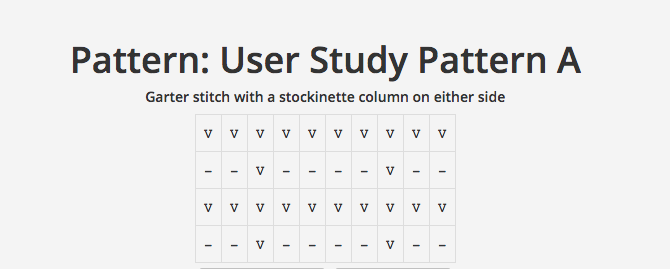
\includegraphics[width=4in]{nonresponsive_pattern_A}

\clearpage

\subsubsection{PurlPal}

\textbf{Responsive Interface Example} \label{responsive}

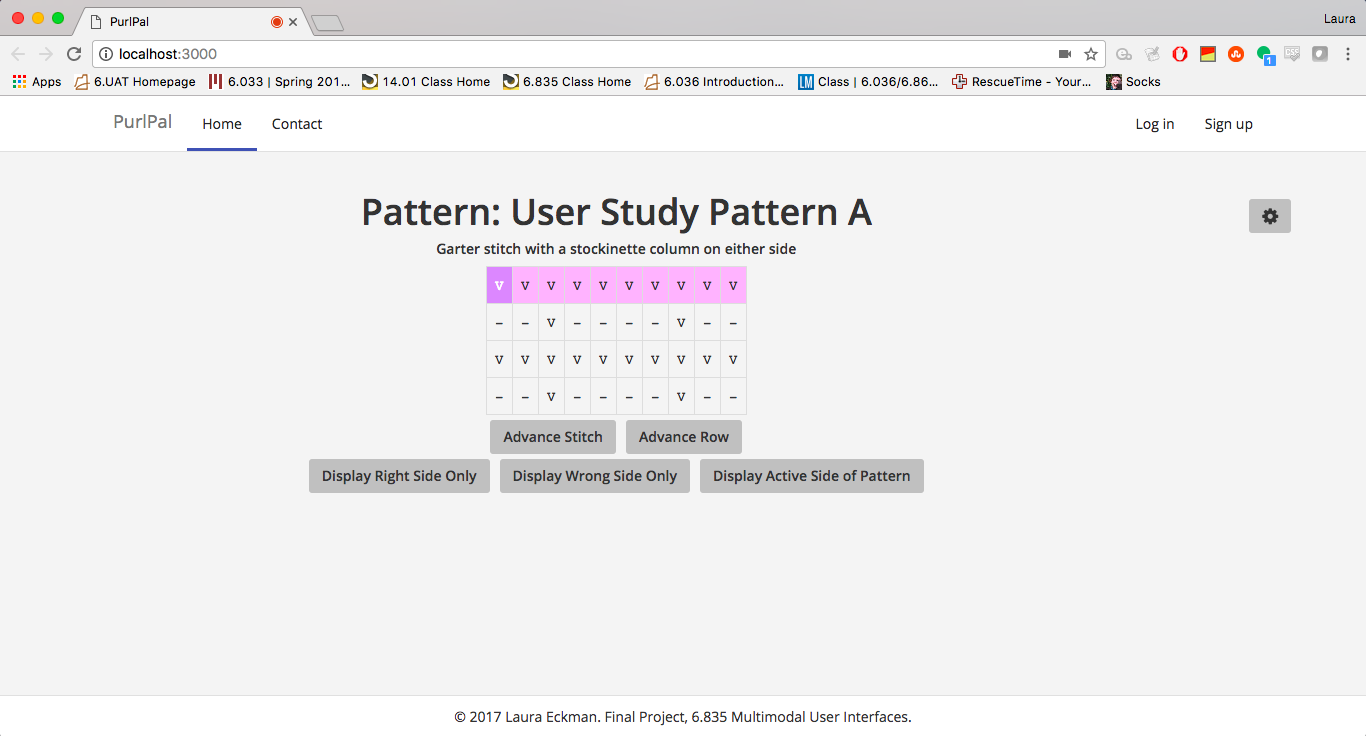
\includegraphics[width=6in]{responsive_pattern_A}

\medskip

\qquad \textbf{Description of Interface - Script} \label{script}

\medskip

\fbox{%
  \parbox{\textwidth}{%

  \medskip
    This is PurlPal!

    \medskip

    PurlPal will track your knitting as you move through the pattern using this sensor.
    The sensor is not perfect, so you can also navigate through the pattern by using voice commands like ``move forward'' to go to the next stitch or ``next row'' to move to the beginning of the next row.
    You can also use these buttons or double click on any stitch to jump anywhere in the pattern.

    \medskip

    By default, PurlPal shows a chart of how the pattern looks from the right side.
    You are also welcome to look at the chart from the wrong side, or toggle between the right side and wrong side as you knit, by using these buttons.

    \medskip

    If you want to turn off motion detection or voice recognition, or you want to see available voice commands, you can find those in the settings menu here.

    \medskip

    Please get into position to start knitting so I can calibrate the sensor - but don't actually start yet.
    \\ ** calibrate sensor *
    \\ Okay, you can begin now. \medskip

  }%
}

\subsection{PurlPal Questionnaire} \label{questionnaire}

\fbox{%
  \parbox{\textwidth}{%
    %\begin{center}
    \begin{enumerate}
      \item I found PurlPal easy to use. \\ \\
      Very True \quad Mostly True \quad Slightly True \quad Slightly False \quad Mostly False \quad Very False
      \item I preferred navigating with speech rather than my mouse. \\ \\
      Very True \quad Mostly True \quad Slightly True \quad Slightly False \quad Mostly False \quad Very False
      \item I preferred navigating with speech rather than motion detection. \\ \\
      Very True \quad Mostly True \quad Slightly True \quad Slightly False \quad Mostly False \quad Very False
      \item I preferred navigating with motion detection rather than my mouse. \\ \\
      Very True \quad Mostly True \quad Slightly True \quad Slightly False \quad Mostly False \quad Very False
      \item I would use a system like PurlPal for complex patterns only. \\ \\
      Very True \quad Mostly True \quad Slightly True \quad Slightly False \quad Mostly False \quad Very False
      \item I would use a system like PurlPal for simple patterns only. \\ \\
      Very True \quad Mostly True \quad Slightly True \quad Slightly False \quad Mostly False \quad Very False
      \item I prefer the row counting feature over tracking my place within the row. \\ \\
      Very True \quad Mostly True \quad Slightly True \quad Slightly False \quad Mostly False \quad Very False
      \item I preferred knitting with PurlPal more than with the non-responsive pattern. \\ \\
      Very True \quad Mostly True \quad Slightly True \quad Slightly False \quad Mostly False \quad Very False
      \\ \\ \\
      What features would you like to see added to PurlPal?
      \\ \\ \\ \\
      What, if any, features of PurlPal did you find unnecessary?
      \\ \\ \\ \\
      General Feedback:
      \\ \\ \\ \\
    \end{enumerate}
    %\end{center}
  }%
}


\end{document}
